% Consider how you might describe the drawing or block tower in Figure \ref{fig:task}A. Both images could be described in language that carves up the image, intuitively, at multiple levels of abstraction -- how would you choose between describing the drawing using a simple but low-level vocabulary of basic strokes (like \textit{lines, circles, and squares}) vs. a set of names for some of its functional parts (like \textit{antenna} or \textit{dial}); or between describing the block tower as composed of \textit{red blocks} and \textit{blue blocks} vs. of higher-level parts like a \textit{roof} and \textit{floors}?

% All we know about this dataset is that it has STRUCTURE; what we expose is variation in nameability. 

% Extend from holistic judgements and labeling to more detailed descriptions of object structure.
% lots of parts
% lots of structure

% We begin by developing a large dataset of two domains of hierarchical object stimuli (Fig. \ref{fig:task}A) and a procedural language experiment to elicit human descriptions of each object.
% In this section we investigate the basic claim that people are able to flexibly describe object structure, and establish a correspondence between linguistic descriptions and conceptual representations.
% While the overarching aim of this paper was to investigate how people talk about the compositional structure of objects, we also wanted to explore how context affects the concepts we use to represent and talk about objects-- particularly the level of abstraction our concepts occupy.
% We therefore needed a set of stimuli that a) had varied compositional structure, b) could be divided into multiple distinct categories (i.e. contexts), and c) was constructed from a set of simple elements that could be combined at various levels of abstraction.

% How do people describe the compositional structure of complex objects across varied domains?
% And how does context affect the level of abstraction that people use to represent objects?
% To study these questions, 

A core motivation for this work is to propose and validate a general approach to identifying the library of part concepts that people invoke to decompose objects.
Towards this end, we needed a sufficiently large and varied collection of objects, and a naturalistic task for eliciting detailed descriptions of their structure. 

% To gain traction on the question of how people robustly communicate about object structure, we first developed a large and varied collection of structured object stimuli and elicited natural-language descriptions of them. % (Fig.~\ref{fig:task}A).
% In this section, we describe our stimulus  and task procedure, and evaluate a basic correspondence between the language participants used to describe our stimuli and the program representations that underlie their construction.

\subsection{Methods}

\paragraph{Participants}
465 participants recruited from Prolific completed the task. 
Participants provided informed consent and were paid approximately \$15 per hour. % for their time.

% (A) Example linguistic descriptions for objects from each domain. (B)
% \textbf{TODO: Add back examples as panel A on the left, but with substantial compression. Re-format text by concatenating what/where content.} 
\begin{figure*}[ht!]
  \begin{center}
  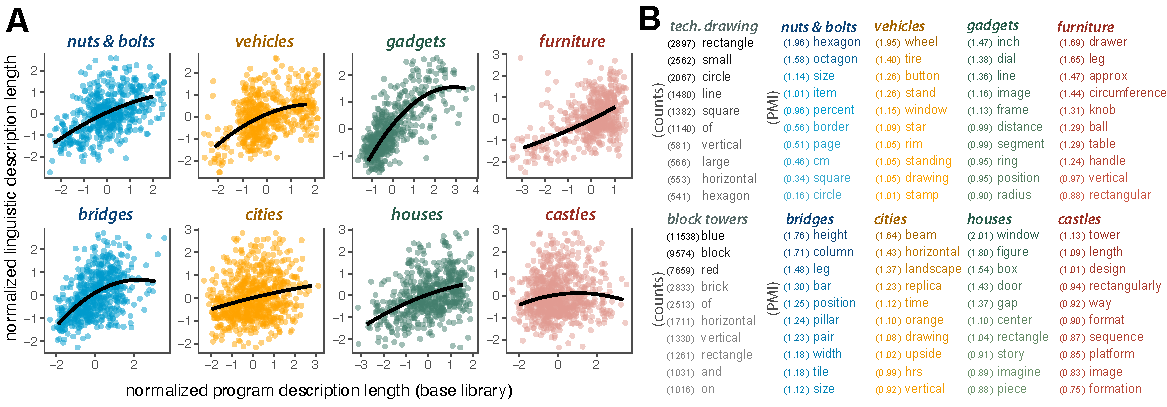
\includegraphics[width=0.99\linewidth]{figures/lax_description_length_and_word_distribution.pdf}
  \caption{(A) Relationship between length of base-library programs and length of linguistic descriptions. (B) \textit{Left:} Top-10 words that appeared most frequently in descriptions for each domain. \textit{Right:} Top-10 words with highest pointwise mutual information (PMI) within each subdomain.}
  \label{fig:words}
  \end{center}
\end{figure*}

\paragraph{Stimuli} 

% To accomplish this, we constructed two domains of stimuli-- (\textit{technical drawings} and \textit{block towers}) (Fig. \ref{fig:task}A)-- that are each generated from a shared base set of procedural, symbolic primitives (shapes or blocks).
% We then ran an experiment to elicit language from subjects who were familiarized with stimuli from a specific \textit{subdomain}-- each containing items generated from distinct generating procedures over these primitives and varying hierarchically in terms of their compositional parts.
% We hypothesized that the vocabularies people used to describe each stimulus would be \textit{context-specific}: that participants would tend to use different vocabularies tailored to the subdomain distribution of stimuli they were shown.

% different motivation for artificial stimuli: XXX
% Don't need to talk about nameability: say it has structure
% We expose variability in structure (x-axis in part II)
% While many such categories exist in the real world, these often come with canonical ways of being decomposed into parts, or have a hierarchical structure that is too ambiguous to permit the formal modeling approach of \ref{sec-part-ii}.

% To construct a set of stimuli with variation in compositional structure, 

% todo: tie to program abstraction
% Desiderata: 1) varied set of categories, 2) hierarchical structure; 3) primitives + higher-order abstractions available to describe, 4) novel + evocative
% 	What do these buy us?
% #1 more general findings
% #2 reminiscent of hierarchical structure of real-world concepts
% #3 allows us to test the notion of "basic-level" but for parts (Rosch et al.) (“just right” level of abstraction)
% #4 lets us look at learning (later)
% why drawings? why block towers?

To ensure that we had a sufficiently large and diverse collection of objects, we developed a hierarchical procedure for synthesizing complex configurations of shapes. 
Taking inspiration from recent work employing line drawings and block towers to investigate how people learn and represent the compositional structure of objects \shortcite{tian2020learning, mccarthy2021learning,wang2021learning}, we defined two stimulus \textit{domains}, distinguished by the set of base shape primitives used to generate them (Fig.~\ref{fig:task}A).
\textit{Drawings} are composed of simple geometric curves (i.e., \texttt{line}, \texttt{circle}) and are evocative of familiar object categories; \textit{Towers} are composed of rectangular blocks (i.e., horizontal and vertical dominoes) and are evocative of simple architectural models.
% These domains were selected for the possibility of evoking consistent interpretations (and therefore part decompositions) across individuals, despite each item ultimately being a novel arrangement of simple primitives.

To investigate the degree to which people invoked category-specific part concepts to describe these objects, rather than the same set of ``atomic'' base primitives in all cases, we further defined four \textit{subdomains} nested within each domain. 
Within \textit{Drawings}, these were informally designated as \textit{nuts \& bolts}, \textit{vehicles}, \textit{gadgets}, and \textit{furniture}; and within \textit{Towers}, as \textit{bridges}, \textit{cities}, \textit{houses}, and \textit{castles} (Fig.~\ref{fig:task}A).
For each subdomain, we procedurally generated 250 unique examples, hierarchically composing the base primitives into increasingly complex, recursively defined parts. 
A \texttt{dresser}, for example, is composed of \texttt{drawers}, which are in turn composed of a \texttt{panel} and \texttt{knobs}, themselves defined by combining \texttt{circles} and \texttt{lines}.
In sum, this procedure yielded a collection of 2000 objects spanning a wide range in complexity: 1000 Drawings and 1000 Towers, each accompanied by a graphics program that can be used to regenerate it in terms of the base primitives.

% Alongside each stimulus, generative models also emitted a corresponding \textit{program}, expressed in a domain-specific language, that fully specified a procedure for recreating the stimulus from the set of base primitives shared across its \textit{domain}.
% We enumerated stimuli for each subdomain, and selected a random but biased sample of each to obtain 250 stimuli of varying complexity for each subdomain.

% two domains were further divided into four \textit{subdomains}, each defined by a distinct generative model that was hand-designed to produce objects of a recognizable subordinate category (e.g., \textit{furniture}, \textit{castle}) from a set of predefined abstractions (e.g., \textit{legs}, \textit{towers}).

% Our stimulus set was divided into two distinct \textit{domains}, each procedurally generated from a different set of base primitives (Fig.~\ref{fig:task}A):
% \textit{technical drawings} were designed to resemble schematic drawings of functional objects and were composed of simple geometric shapes; 
% \textit{block towers} were designed to resemble simple architectural models and were composed of 2D rectangular blocks.
% Each of the two domains were further divided into four \textit{subdomains}, each defined by a distinct generative model that was hand-designed to produce objects of a recognizable subordinate category (e.g., \textit{furniture}, \textit{castle}) from a set of predefined abstractions (e.g., \textit{legs}, \textit{towers}).

% Generative models consisted of a set of nested, parametric functions operating over the base primitives, hierarchically composing them into increasingly complex, recursively-defined parts.
% A \textit{dresser}, for example, is composed of \textit{drawers}, which are in turn composed of a \textit{panel} and \textit{knobs}, and which are defined finally over a shared set of simple shape primitives.
% Alongside each stimulus, generative models also emitted a corresponding \textit{program}, expressed in a domain-specific language, that fully specified a procedure for recreating the stimulus from the set of base primitives shared across its \textit{domain}.
% We enumerated stimuli for each subdomain, and selected a random but biased sample of each to obtain 250 stimuli of varying complexity for each subdomain.

\paragraph{Task procedure}

Each participant was instructed to provide step-by-step instructions for how to ``draw'' or ``build'' 10 different ``drawings'' or ``models'' sampled from a \textit{single} subdomain.
% , such that someone else could reconstruct each one based on their instructions.
% Each participant produced descriptions for 10 items drawn from a single \textit{subdomain} (e.g., only \textit{castles}). 
% To gain familiarity with the task-relevant distribution of stimuli and part abstractions, participants first clicked through 25 images of other stimuli from the same subdomain.
At the start of each session, participants were first familiarized with the general characteristics of the subdomain by viewing 25 examples (none of which then appeared during the main experiment).
Throughout the session, they were also shown the upcoming 7 objects they would be asked to describe, to provide them with concurrent information about how objects varied within the subdomain.
% However participants were not encouraged to produce instructions that disambiguated their items from others in their domain, as in a traditional reference game.
Because we were primarily focused on interrogating which part descriptors people invoke, we designed the text-entry interface to encourage participants to describe each step by composing a \textit{what}-phrase and a \textit{where}-phrase, which were entered into separate text boxes. 
Participants could include as many instruction steps as they deemed necessary and there was no trial time limit.

% which  language referring to parts distinct from language referring to spatial relations. 
% \textit{what} they would draw/place \textit{where}
% designed the text-entry interface with two separate : a \textit{where} 
% the language used to refer to the parts of an object from spatial descriptions of where those parts should go, participants typed each step of their procedure into a pair of \textit{what} and \textit{where} text boxes, describing what should be drawn/placed where, in order, to reproduce the target image. 

\paragraph{Language preprocessing} % spacy, en_core_web_lg,
To investigate the content of the instructions generated by participants, we used the spaCy NLP library to extract and lemmatize words, including part-of-speech (POS) tagging to remove determiners and punctuation. We also replaced common typos (``sqaure,'' ``cirlce,'' etc.) and spelling variations (``centre,'' ``colour,'' etc.) with their canonical spellings in US English.

\subsection{Results}
% ($b=XXX$, $t=XXX$, $p=XXX$)
% $XXX\%$ (95\% CI: $[XXX, XXX]$)

\paragraph{People use more words to describe more complex objects (up to a point)}
% We first set out to establish whether participants' language was sensitive to the distribution of objects they were describing.
% The high degree of variation in stimulus complexity provided a natural opportunity to explore the relationship between the relationship between the number of simple shape elements in an object and how many words participants used to describe it. 
%%%%%%% 
% We ran a linear mixed effects models with fixed effects for domain and trial number, an interaction term between the two, as well as random intercepts for subdomain and participant.
% \textit{Block tower} instructions were longer than those for \textit{technical drawings}, both in terms of the number of \textit{what-where} steps  ($b=5.08$, $t=10.9$, $p<0.001$) and raw character counts ($b=373$, $t=8.24$, $p<0.001$). 
% We suspected that this was due to participants identifying a greater number of distinct entities in the \textit{block tower} stimuli, which was supported by a greater number of words entered in the \textit{what} boxes of \textit{block towers} than for \textit{technical drawings} ($b=25.8$, $t=9.55$, $p<0.001$).
% Together, these results confirm that participants' descriptions were sensitive to the kinds of items they were describing, but what about the stimuli themselves explains this variation in language? 
%%%%%%%
The high degree of shape variation in our stimulus set provided us with a natural opportunity to explore the relationship between the complexity of an object and the length of the linguistic description participants provided for it.
Insofar as participants display a tendency to decompose objects into a consistent number of parts, regardless of how complex these parts are, the length of their descriptions would be predicted to remain stable over a wide range in object complexity. 
Alternatively, if participants tend to decompose objects into a set of commonly recurring parts, and provide a description for each one, the length of their descriptions would be predicted to positively correlate with object complexity. 
A third possibility is that there is a systematic but non-linear relationship between object complexity and linguistic description length \cite{sun2021seeing}, consistent with a compromise between the first two strategies. 
% has suggested a systematic but non-linear relationship between this measure of  object complexity and the length of their linguistic descriptions \cite{sun2021seeing}.
% , which was consistent with initial observations in our data (Fig. \ref{fig:words}A).
% To test this hypothesis more rigorously, we operationalized natural-language description length using the mean number of words entered in the \textit{what} text boxes and operationalized the program length as the number of tokens required to express that object in the base DSL.
% To test this hypothesis more rigorously, we fit a mixed-effects model to predict the length of each natural-language description, including fixed effects of the object's subdomain (with eight levels) and the corresponding program length in the base DSL.

For these analyses, we operationalize object complexity as the length of the graphics program that generated it using the base primitives and measure the length of linguistic descriptions as the number of words provided in the \textit{what} phrases only.
To tease apart the above possibilities, we fit a mixed-effects model to predict linguistic description length from graphics program length (Fig. \ref{fig:words}A), including random intercepts for participants and random effects of program length at the participant level.
% and effects of program length at the participant-level. %the number of program tokens required to recreate the object (Fig. \ref{fig:words}A).
We observed a significant main effect of program length ($t(318)=14.8, p < 0.001$ across all subdomains), providing strong evidence against the view that participants invoke part concepts of arbitrary complexity in order to provide instructions of the same length. 
We also found that a model including an additional quadratic effect of program length, allowing for a non-linear relationship, significantly improved the fit ($\chi^2(3)=38.6$), although the strength of this relationship varied across subdomains.
These findings suggest that people generally use more words to describe more complex objects, but the strength and nature of this relationship can vary widely across object categories. 
% Moreover, even the best-fitting quadratic model failed to capture a large proportion of the variation in language using only program length as a measure. % written only in terms of simple shape primitives.

% Nevertheless, it appeared that instructions produced for both domains spanned a range of levels of abstraction (Fig. \ref{fig:words} A), with some referring to lower level primitives (i.e. geometric shapes and individual blocks) and some to more abstract compositions of these lower elements (e.g. ``desks'', ``pillars'', and ``castle-like block towers'').
% Stimuli from each domain were constructed from distinct sets of base primitives that can be combined according to distinct sets of constraints, allowing us to investigate whether participants systematically varied their vocabulary according to their context.

% n_steps ~ domain * trial_num + (1 | subdomain) + (1 | gameID)
%                              Estimate Std. Error         df t value Pr(>|t|)    
% (Intercept)                   4.36409    0.33821    8.47840  12.904 7.25e-07 ***
% domainstructures              5.07991    0.46552    7.58715  10.912 6.61e-06 ***
% trial_num                    -0.06105    0.02143 4183.00156  -2.848  0.00442 ** 
% domainstructures:trial_num   -0.29242    0.02878 4183.00156 -10.162  < 2e-16 ***


% char_sum ~ domain * trial_num + (1 | subdomain) + (1 | gameID)
% Fixed effects:
%                           Estimate Std. Error       df t value Pr(>|t|)    
% (Intercept)                 305.566     32.635    7.475   9.363 2.16e-05 ***
% domainstructures            373.091     45.288    6.922   8.238 8.04e-05 ***
% trial_num                    -5.493      1.640 4182.994  -3.350 0.000817 ***
% domainstructures:trial_num  -29.624      2.201 4182.994 -13.457  < 2e-16 ***


% n_whats_filtered ~ domain * trial_num + (1 | subdomain) + (1 |      gameID)
%                             Estimate Std. Error        df t value Pr(>|t|)    
% (Intercept)                  17.6224     1.9618    7.9137   8.983 2.01e-05 ***
% domainstructures             25.8495     2.7060    7.1447   9.553 2.53e-05 ***
% trial_num                    -0.2667     0.1174 4182.9953  -2.272   0.0231 *  
% domainstructures:trial_num   -1.5601     0.1576 4182.9953  -9.900  < 2e-16 ***


\paragraph{People use different words to describe different objects} % Looking at content rather than length

While none of the items in our stimulus set look exactly like real-world objects and buildings, several of them are nevertheless \textit{evocative} of familiar visual categories (e.g., vehicles, furniture, houses). 
Insofar as these associations guided their language behavior to some extent, participants may have used different words to describe the parts of objects from different subdomains. 
Alternatively, if people referred exclusively to low-level shape primitives common to all subdomains within a given domain, then we would not expect there to be large differences in the relative frequency of words people produced. 
To explore these possibilities, we aggregated tokens produced by all participants for objects in each subdomain and computed the pointwise mutual information (PMI) for each word, providing initial insights into the strength of association between a given word and subdomain (Fig.~\ref{fig:words}B).
% We aggregate the preprocessed instructions across each subdomain and compute the pointwise mutual information (PMI) of each word with respect to each subdomain (as opposed to the full domain; we consider the domains independently.) 
% These PMI values were estimated using a Laplace smoothing metric to eliminate extremely low-frequency words (n $\leq$ 5). %; full analysis code is released at the code repository.
This analysis revealed several words that were used often within a particular subdomain, but not in others (e.g., \textit{drawer}, \textit{leg}, and \textit{knob} in the \textit{furniture} subdomain), suggesting that certain part concepts may be specific to certain subdomains.

%%% JSD analysis
To rigorously evaluate whether the presence of these highly diagnostic words reflected more general differences in word usage across subdomains, we computed the Jensen-Shannon distance (JSD) between the word frequency distributions from each set of subdomains, aggregating across all trials in that subdomain.
We compared the the mean of all pairwise JSDs to a null distribution generated by randomly assigning trials to subdomain groups and found that the distance between subdomains was greater than that expected under the null (\textit{Drawings}: $d = 0.439$, $p < 0.001$; \textit{Towers}: $d = 0.328$, $p < 0.001$), providing strong evidence that participants used different words to describe objects in different subdomains.
% The larger JSD values for Drawings further suggest that the subdomains of Drawings elicited more distinct descriptions compared to those of Towers. %any interpretation needed here?
% DOMAIN-LEVEL JSD: To estimate how dissimilar language was across domains, we computed the Jensen-Shannon distance (JSD) between the word frequency distributions aggregated across all trials in each domain, and compared this value to a null distribution of random assignments of trials to domains.
% We found that the distance between word distributions at the domain-level was significantly greater than would be expected by chance ($d = 0.736$, $p<  0.001$).
% Similarly, when we instead aggregated over subdomains, we found that mean distance between subdomains was significantly greater than between random assignments to subdomains (\textit{Drawings}: $d = 0.439$, $p < 0.001$; \textit{Towers}: $d = 0.328$, $p < 0.001$).
Taken together, these analyses indicate that people used a wide variety of terms to describe otherwise visually similar objects, in many cases referring to parts of real-world objects, rather than to simple graphics primitives.

% This is further supported by computing the F-statistic to measure within-cluster variance, comparing word-count vectors labeled with a given subdomain to randomly-assigned subdomain labels. 

% However, examining the relative word frequency distribution produced greater discriminability by subdomain for \textit{technical drawings} ($\Delta F = 12.5$, 95\% CI: [$9.46$, $16.0$], $p<0.001$) than for {block towers} ($\Delta F = 1.47$, 95\% CI: [$0.0441$, $2.83$], $p=0.088$). 

% We find that the \textit{technical drawing} subdomain labels explain cluster variance signficantly better than random assignments ($\Delta F = 12.5$, 95\% CI: [$9.46$, $16.0$], $p=0$); this effect is not significant for subdomain labels in the \textit{block towers} domain ($\Delta F = 1.47$, 95\% CI: [$0.0441$, $2.83$], $p=0.088$).

% We conduct a preliminary linguistic analysis of subdomain-level vocabulary variation. 

% Fig. \ref{fig:vocabulary_gallery}A (left, black) shows the top 10 words ordered by their \textit{base counts} across each whole domain, contrasted by the top-10 words ordered by \textit{PMI} for each subdomain (right columns, colored), indicating the usage of words (eg. \textit{drawer}, \textit{leg}, and \textit{knob} in the \textit{furniture} subdomain) suggestive of subdomain-specific part structure. 

% Fig. \ref{fig:library_gallery}B also shows TSNE-visualizations of word-count vectors constructed for each stimulus, suggesting that there may be greater subdomain-level language differentation in the \textit{technical drawings} domain than in the \textit{block towers} domain. This is further supported by computing the F-statistic to measure within-cluster variance, comparing word-count vectors labeled with a given subdomain to randomly-assigned subdomain labels. We find that the \textit{technical drawing} subdomain labels explain cluster variance signficantly better than random assignments ($\Delta F = 12.5$, 95\% CI: [$9.46$, $16.0$], $p=0$); this effect is not significant for subdomain labels in the \textit{block towers} domain ($\Delta F = 1.47$, 95\% CI: [$0.0441$, $2.83$], $p=0.088$).
